\chapter{Fonctions}

\section{Introduction}

En mathématique, nous travaillons avec des objets. Nous avons déjà vu plusieurs de ces objets, tel que les nombres, les figures géométriques, les opérations, les ensembles, etc. Un object particulièrement utile en mathématique s'appelle une fonction. Une fonction est une relation entre deux ensembles, qui ``relie'' des éléments du premier ensemble (le ``domaine'') au second ensemble (``l'image'').

\begin{center}
	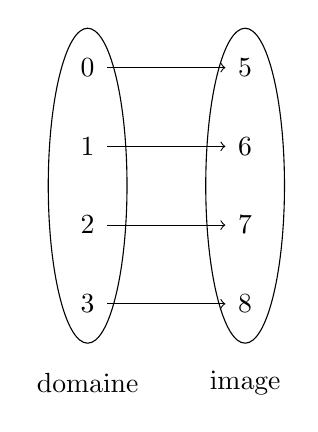
\begin{tikzpicture}
        \draw node at (0,0)  {0};
        \draw node at (0,-1) {1};
        \draw node at (0,-2) {2};
        \draw node at (0,-3) {3};
        \draw (0,-1.5) ellipse (0.5 and 2);
        \draw node at (0,-4) {domaine};

        \draw node at (2,0)  {5};
        \draw node at (2,-1) {6};
        \draw node at (2,-2) {7};
        \draw node at (2,-3) {8};
        \draw (2,-1.5) ellipse (0.5 and 2);
        \draw node at (2,-4) {image};

        \draw[thin, ->] (0.25,0)  -- (1.75,0);
        \draw[thin, ->] (0.25,-1) -- (1.75,-1);
        \draw[thin, ->] (0.25,-2) -- (1.75,-2);
        \draw[thin, ->] (0.25,-3) -- (1.75,-3);
	\end{tikzpicture}
\end{center}

L'ensemble des flèches dans l'image au-dessus représentent une fonction allant de l'ensemble $\{0,1,2,3\}$ à l'ensemble $\{5,6,7,8\}$.

\section{Écriture d'une fonction}

Nous ne pouvons pas utiliser des dessins pour définir toutes les fonctions que nous utilisons, pour des raisons assez évidentes (manque de place, difficile à généraliser, etc.). Les mathématiciens ont donc du inventer une manière de pouvoir écrire une fonction en language mathématique. Afin de l'illustrer, nous allons travailler avec un example. Considérons l'expression suivante:
\[
    f: \R \to \R, \ \ f(x) = x + 1
\]
La première lettre, $f$, est le nom de la fonction. On le retrouve un peu plus loin aussi. Toute fonction doit avoir un nom: souvent, on appelle les fonctions $f$ ou $g$, mais nous pouvons en nommer \textit{bonjour} ou \textit{nom de fonction}.

Après le nom de la fonction, nous mettons un ``$:$'', pour séparer le nom de la suite. Nous avons ensuite $\R \to \R$, qui est de la forme $\text{\texttt{domaine}} \to \text{\texttt{image}}$. Dans ce cas (comme dans la majorité des fonctions que nous étudierons), le domaine et l'image sont les réels, $\R$.

Ensuite, nous avons de nouveau le nom de la fonction, $f$, suivit d'entre parenthèse une variable, $x$. On met un égal et de l'autre coté, une expression (dans ce cas, $x+1$) qui incorpore la variable pour donner l'image en fonction de l'inconnue.

Dans ce cas, par exemple, l'image de $2$ par cette fonction $f$ est $2+1 = 3$. L'image de $0$ est $0+1 = 1$. Pour écrire ``l'image de $2$ par la fonction $f$'' en language mathématique, on écrit $f(2)$. Nous pouvons donc réécrire ``l'image de $2$ par cette fonction $f$ est $2+1 = 3$'' en language mathématique, ce qui nous donne $f(2) = 2+1 = 3$ ou plus simplement, $f(2) = 3$.

Bien qu'il est important d'inclure le domaine et l'image d'une fonction, étant donné que nous travaillons avec des fonctions qui ont pour domaine et image $\R$, souvent, nous n'incluons pas la partie $f: \R \to \R$, ce qui nous donne simplement $f(x) = x + 1$ comme définition pour la fonction au-dessus.

\vspace{1em}

\begin{exercice}
    Écrit la définition d'une fonction qui retourne comme image son entrée plus 4.
\end{exercice}

\begin{exercice}
    Soit $f(x) = 2x + 3$. Quelle est la valeur de $f(5)$, $f(0)$ et $f(1)$? Pour quelle valeur de $x$ avons-nous $f(x) = 10$? (Indice pour cette dernière question: il faut résoudre une équation.)
\end{exercice}

\section{Vocabulaire pour les fonctions}

Les fonctions sont un nouveau type d'objet, avec cela viennent de nouveaux concepts et un vocabulaire associé.

\begin{definition}
    Une \emph{fonction} est une relation entre deux ensembles qui relie chaque élément du premier ensemble à tout au plus un élément du second ensemble.
\end{definition}

\begin{definition}
    Le \emph{domaine} d'une fonction est l'ensemble des valeurs auxquelles nous pouvons appliquer la fonction.
\end{definition}

\begin{definition}
    L'\emph{image} d'une fonction est l'ensemble des valeurs que l'application de la fonction à des valeurs du domaine peut prendre. Si le domaine de la fonction est $X$, on note l'image de la fonction $f(X)$.
\end{definition}

\begin{definition}
    \emph{L'image d'une valeur par une fonction} est la valeur retournée par une fonction lorsqu'elle est appliquée à un nombre. L'image du nombre $x$ est notée $f(x)$.
\end{definition}

\begin{definition}
    \emph{L'antécédant} d'une valeur par une fonction est la valeur qui doit être donné à la fonction pour obtenir cette image. Si $y$ est cette valeur et que $f(x)=y$, on note l'antécédent de $x$ soit comme $f^{-1}(x)$, soit comme $x$.
\end{definition}

% FIXME: est-ce bien le cas?
\begin{definition}
    Une fonction est \emph{bien-définie} si tous les éléments du domaine ont une image.
\end{definition}